\documentclass{article}
\usepackage{fancyvrb}
\usepackage{fancyhdr}
\usepackage{extramarks}
\usepackage{amsmath}
\usepackage{amsthm}
\usepackage{amsfonts}
\usepackage{tikz}
\usepackage{graphicx}
\usepackage{enumitem}
\usepackage[plain]{algorithm}
\usepackage{algpseudocode}
\usepackage[normalem]{ulem}
\usepackage{hyperref}
\usepackage{xcolor}
\usepackage{caption}
\usepackage{subcaption}
\usepackage{listings}% http://ctan.org/pkg/listings
\lstset{
  basicstyle=\ttfamily,
  mathescape
}

\usetikzlibrary{automata,positioning}

\topmargin=-0.45in
\evensidemargin=0in
\oddsidemargin=0in
\textwidth=6.5in
\textheight=9.0in
\headsep=0.25in

\linespread{1.1}

\pagestyle{fancy}
\lhead{\hmwkAuthorName}
\rhead{\hmwkClass\ (\hmwkClassInstructor\ \hmwkClassTime): \hmwkTitle}
% \rhead{\firstxmark}
\lfoot{\lastxmark}
\cfoot{\thepage}

\renewcommand\headrulewidth{0.4pt}
\renewcommand\footrulewidth{0.4pt}

\setlength\parindent{0pt}

\setcounter{secnumdepth}{0}
\newenvironment{homeworkProblem}[1][-1]{
    \ifnum#1>0
        \setcounter{homeworkProblemCounter}{#1}
    \fi
    \section{Problem \arabic{homeworkProblemCounter}}
    \setcounter{partCounter}{1}
    \enterProblemHeader{homeworkProblemCounter}
}{
    \exitProblemHeader{homeworkProblemCounter}
}

\newcommand{\hmwkTitle}{Assignment\ \#3}
\newcommand{\hmwkClass}{CSE 512}
\newcommand{\hmwkClassTime}{Lecture A}
\newcommand{\hmwkClassInstructor}{Jeffrey Heer}
\newcommand{\hmwkAuthorName}{Emily Gu | Ryan Drapeau | Vimala Jampala}

\title{
    \vspace{2in}
    \textmd{\textbf{\hmwkClass:\ \hmwkTitle}}\\
    \vspace{0.2in}\large{\textit{\hmwkClassInstructor\ \hmwkClassTime}}\\
    \author{\textbf{\hmwkAuthorName\ $\vert$ \hmwkAuthorCSE\ $\vert$ \hmwkAuthorId}}
}

\date{}

\begin{document}

One problem that came up repeatedly when we were exploring our dataset is that there were too many classes for us to create a single visualization. We would have to find a way to filter the data if we wanted it to be easy to view. Accordingly, we designed our visualization to have 26 hyper-links: one for each letter in the alphabet. The page instructs viewers to select the first letter of the department they're interested in.

\begin{center}
    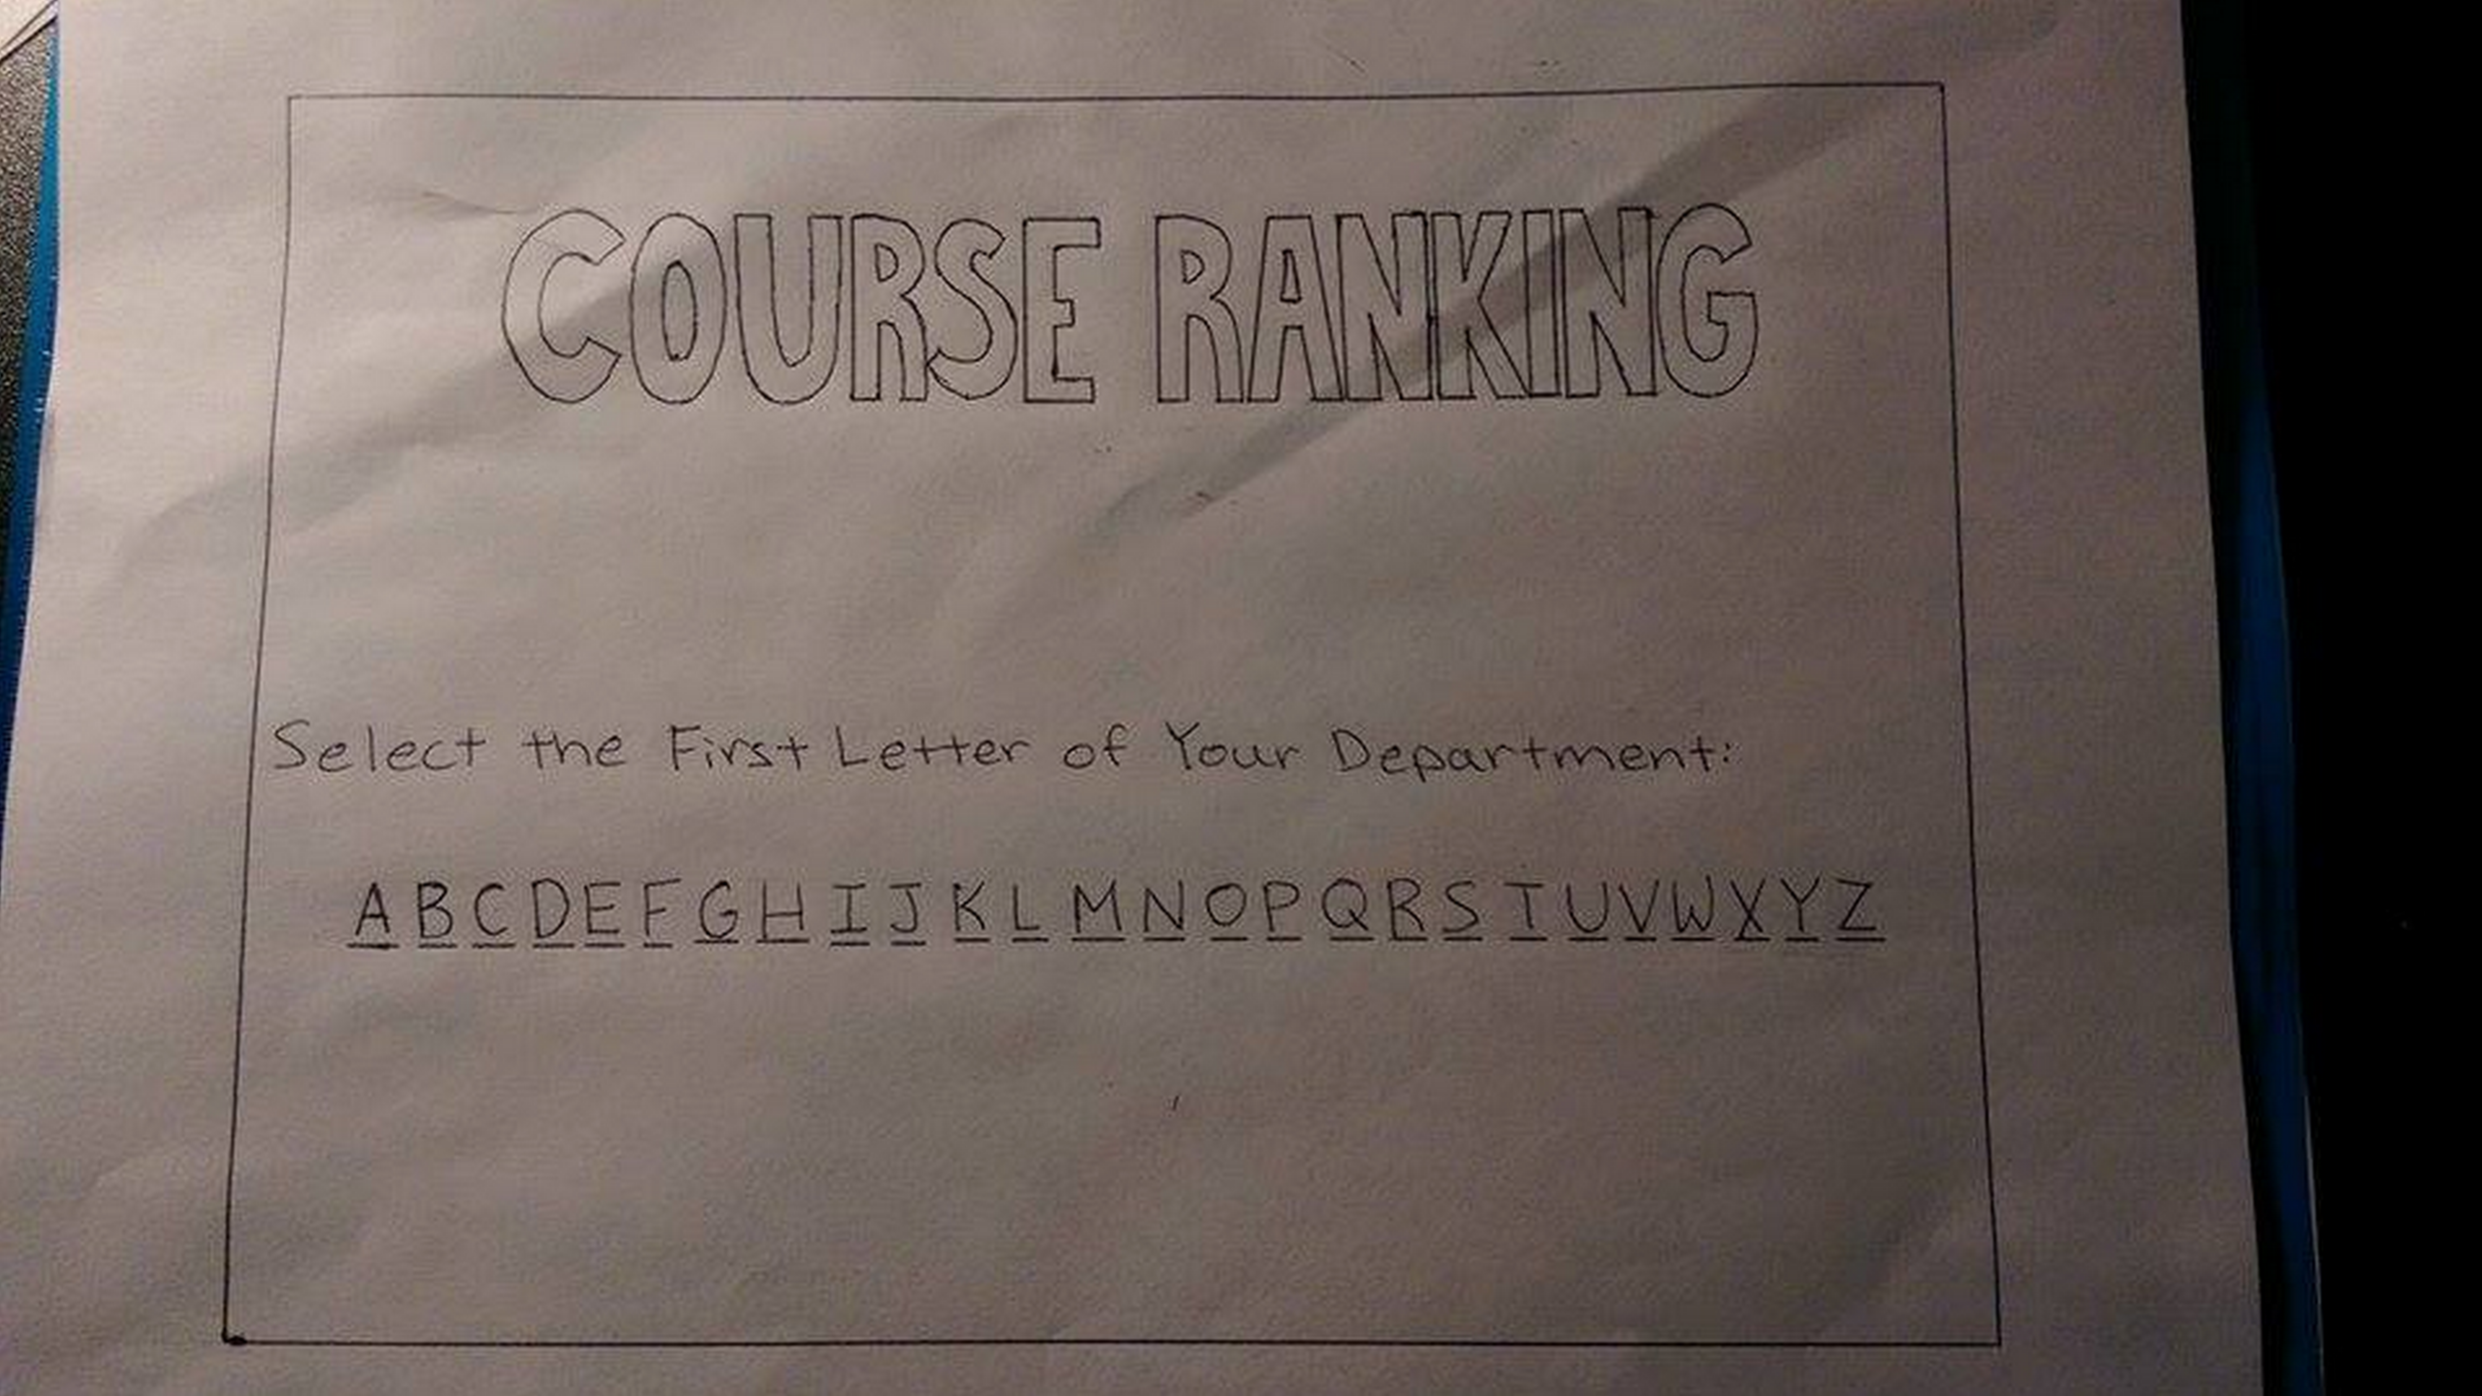
\includegraphics[width=\textwidth]{1.png}
    \captionof{figure}{The landing page of the application.}
\end{center}

Clicking on this letter leads them to another page, with a list of department names:

\begin{center}
    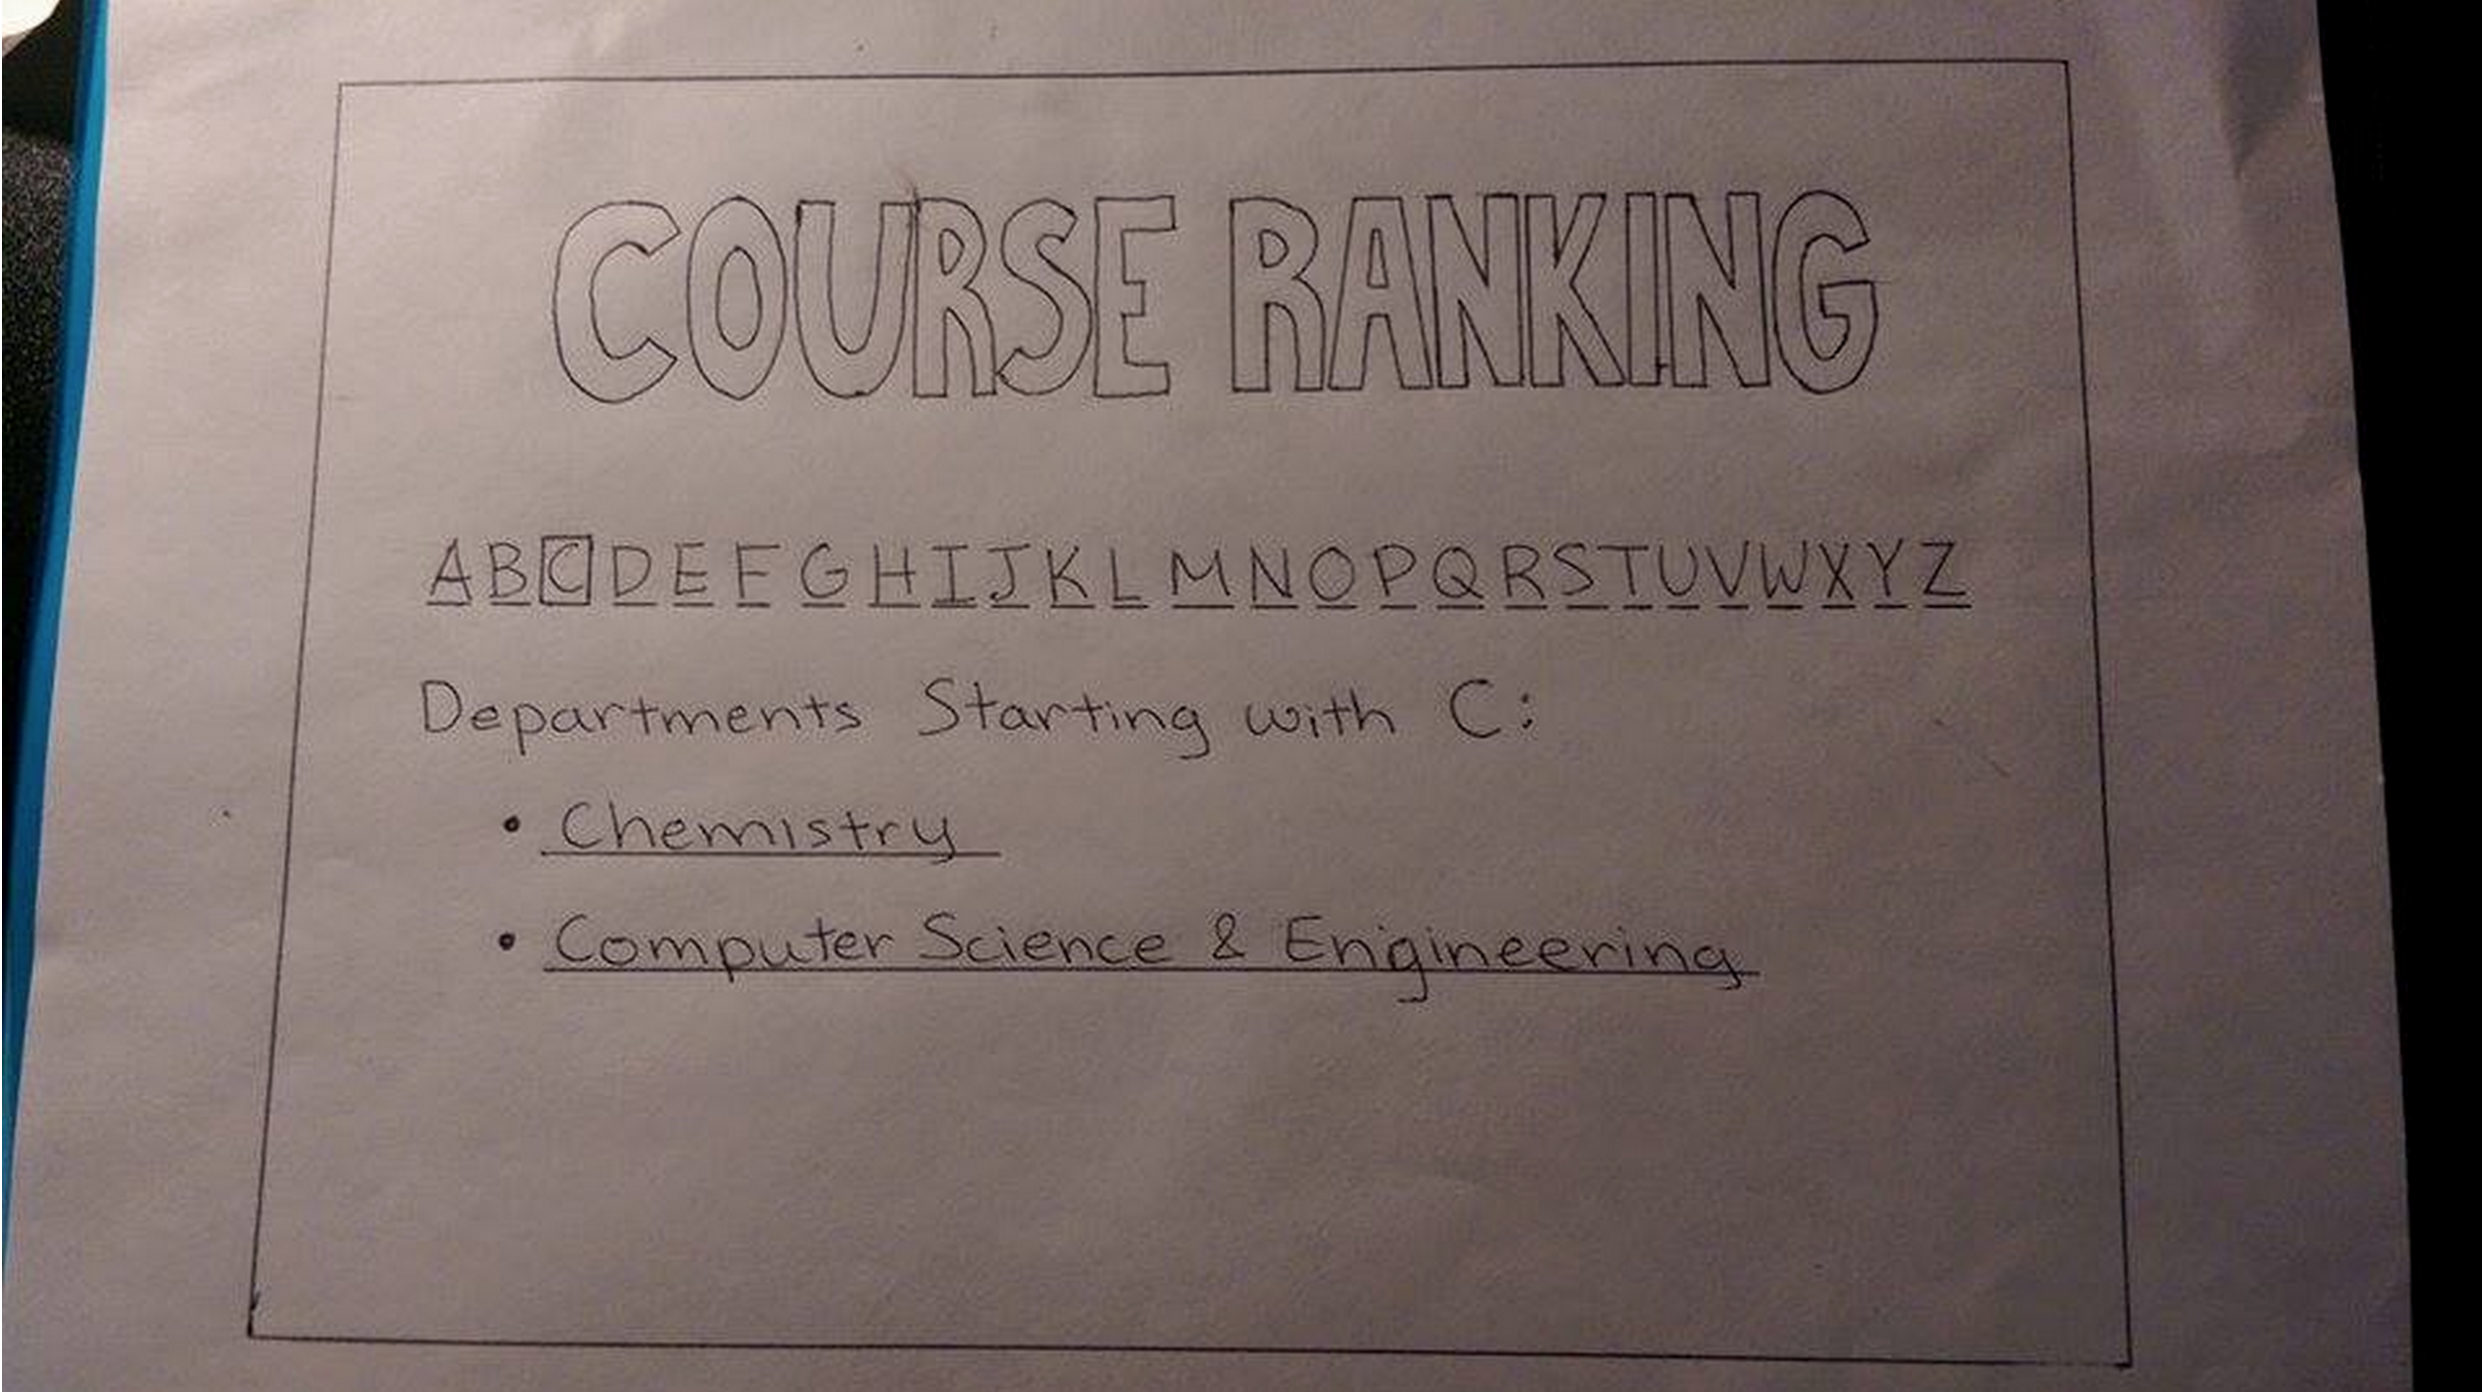
\includegraphics[width=\textwidth]{2.png}
\end{center}

Clicking one of the department names leads them to the following page:

\begin{center}
    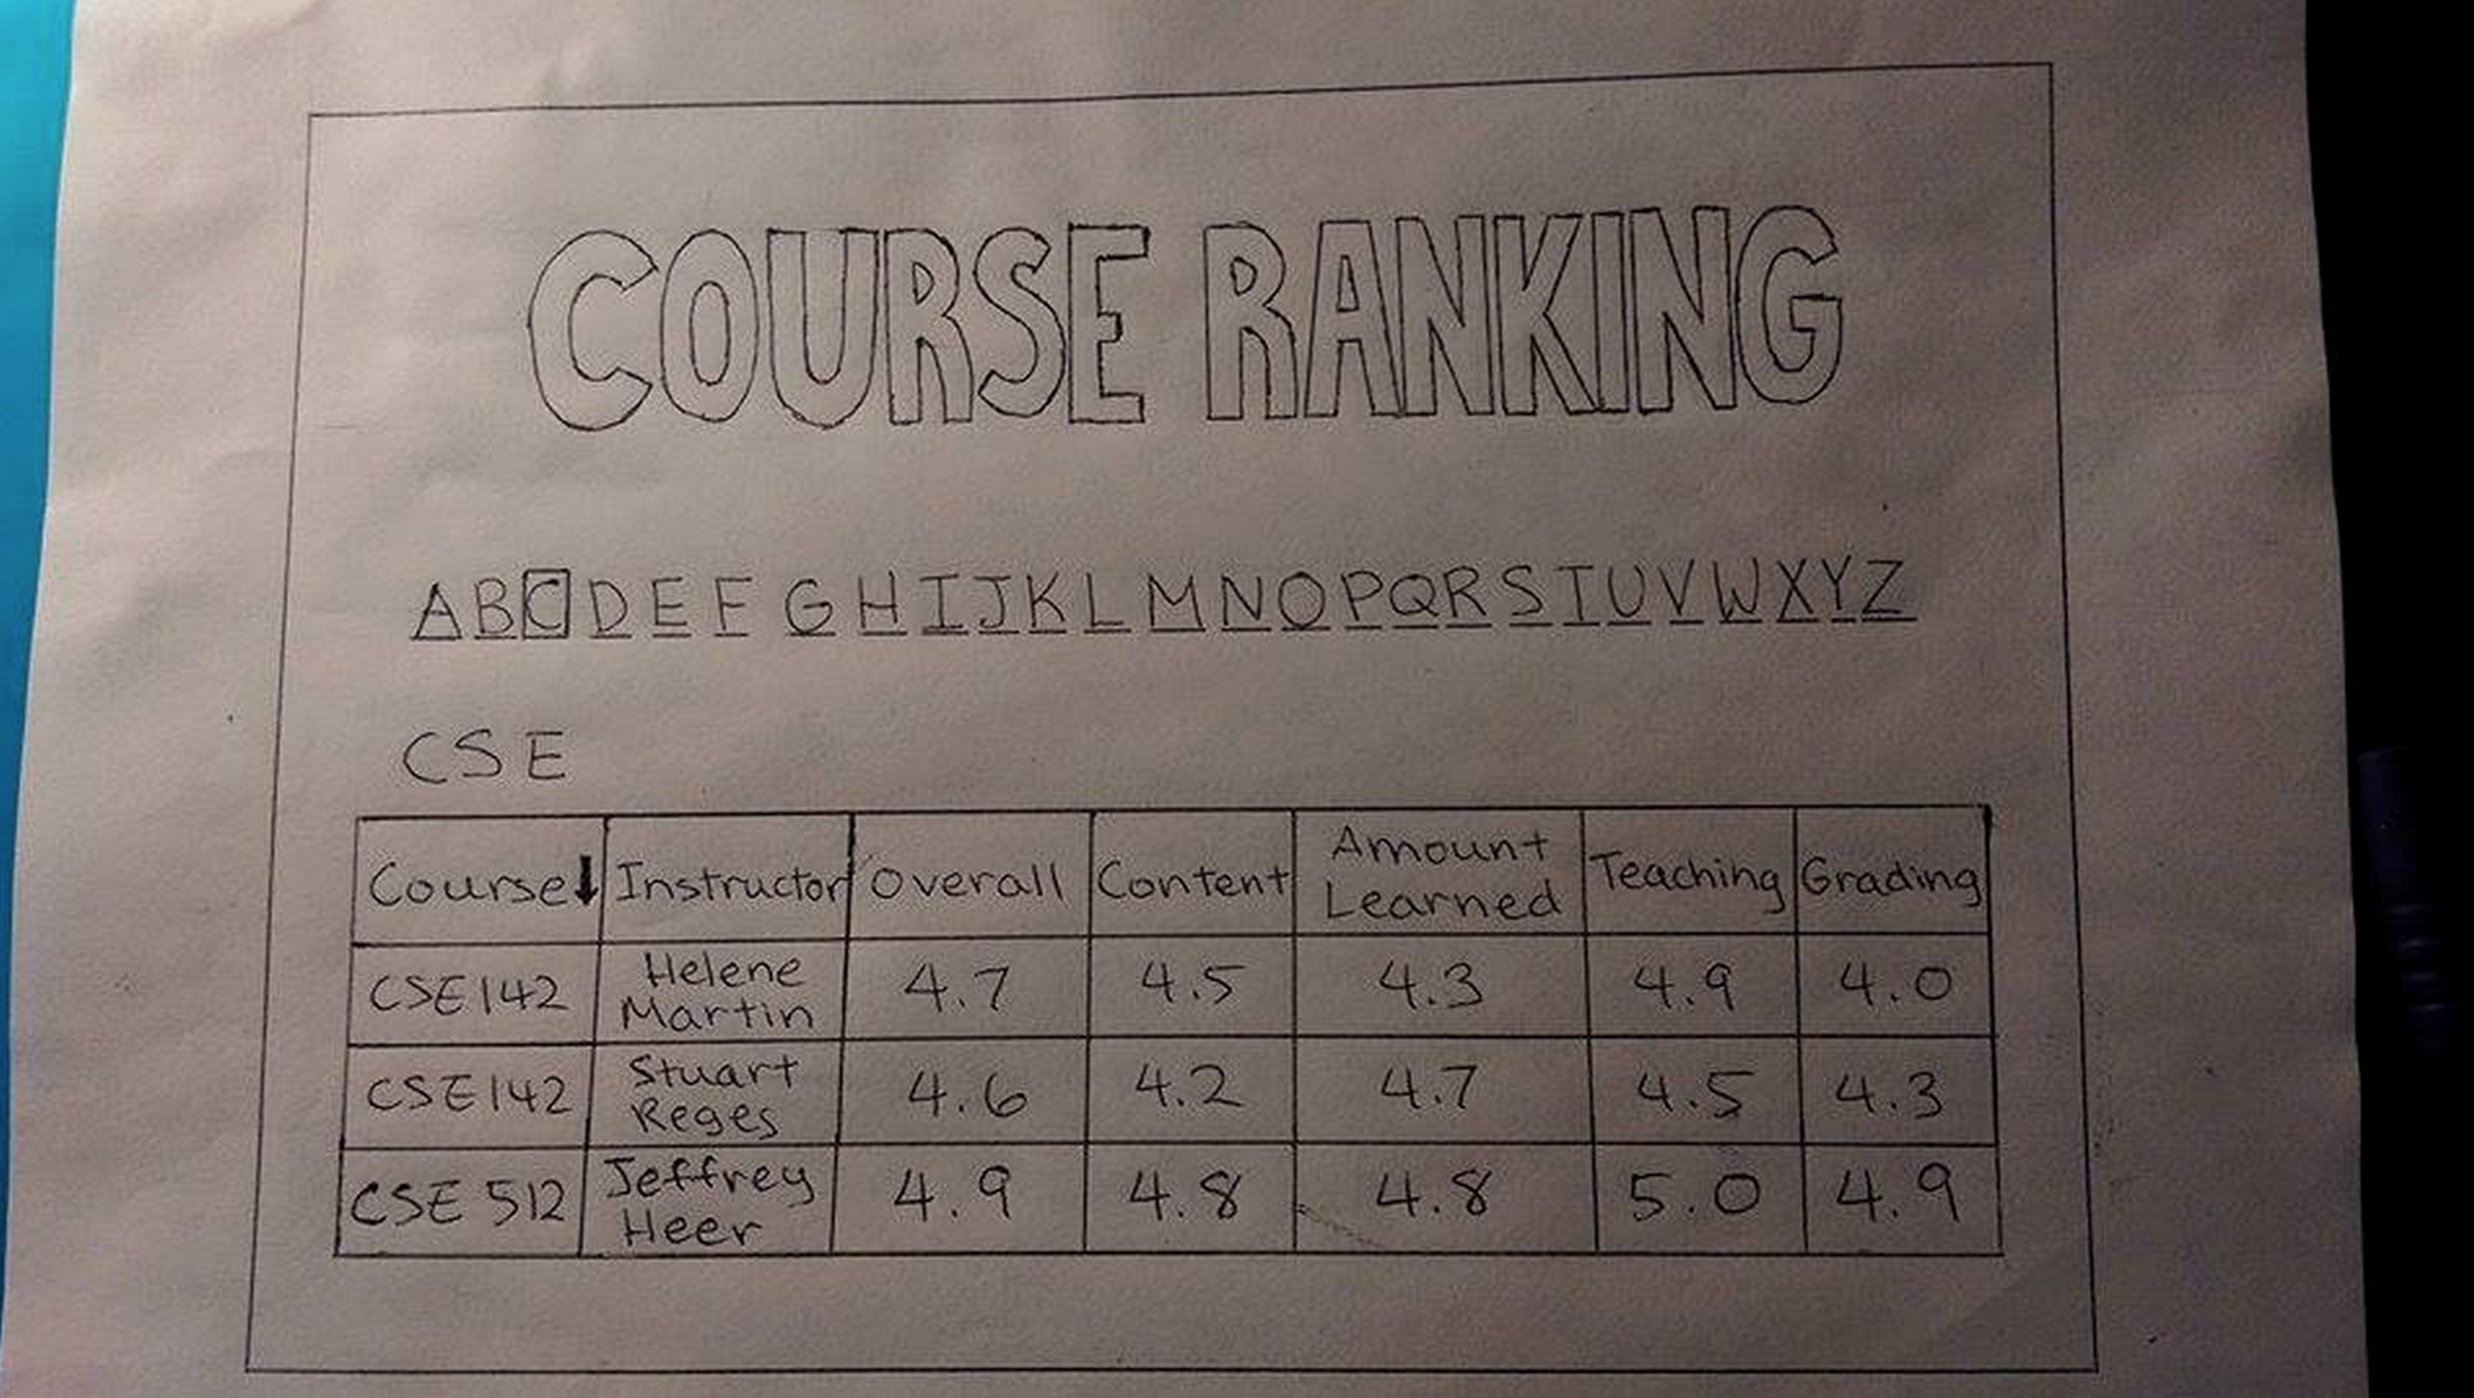
\includegraphics[width=\textwidth]{3.png}
\end{center}

Our next choice was choosing which dimensions to present to the user. After exploring the data, we decided on the following dimensions because they were both dense and the most useful to students:

\begin{itemize}
    \item The course as a whole
    \item The course content
    \item The instructor's effectiveness
    \item The amount learned
    \item The grading technique
\end{itemize}

We were torn between presenting the exact breakdown of each category, and presenting the median vote. On the other hand, providing more data to viewers allows them to learn more and to spot more trends. On the other hand, providing too much data clutters a visualization and makes it hard to interpret.\\

In the end, we decided to only report the median for each category. When we looked at UW's course evaluation catalog, we found there was too much data for us to effectively spot trends and compare classes. By providing only the median value for each category, we provided enough information for users to make an informed choice without cluttering the visualization. Since we were only displaying data for a few dimensions, and since we were only displaying one value per dimension, we decided to use a table to present our data.\\

Once this was done, we brainstormed ways a viewer would want to interact with our visualization. Our intended audience is students searching for classes to register for. Such an audience might want to:

\begin{enumerate}
    \item Choose between two instructors teaching a particular class
    \item Choose between a class taught by one instructor and a different class taught by another class
    \item Decide if they should take a class without knowing which instructor is teaching it
\end{enumerate}

With our current design, a user searching for a particular class would have to either manually scan the page, or use his/her browser's search function to find the class. They would then have to repeat this process if they wanted to look at multiple offerings of the class. Worse still, if a user wanted to search for a combination of class and instructor, they would only be able to manually search the page. They would have to do this for each combination of course and instructor they were interested in.\\

Consequently, we decided to make course numbers and instructor names click-able. Clicking on a course number takes the user to a new page where only information about that course is displayed. This makes learning more about a particular course easy - all a user has to do is find one instance of the course, and then click on it.\\

Similarly, clicking on an instructor's name takes the user to a new page where only courses taught by that instructor are displayed. This makes learning more about a particular instructor much easier. Additionally, these additions make searching for a particular course and instructor combination easy - all a user has to do is search for either the course or instructor, and click on the first link they find. Since our dataset contains a large amount of data, this interaction technique is effective because it allows users to filter data easily.

\begin{center}
    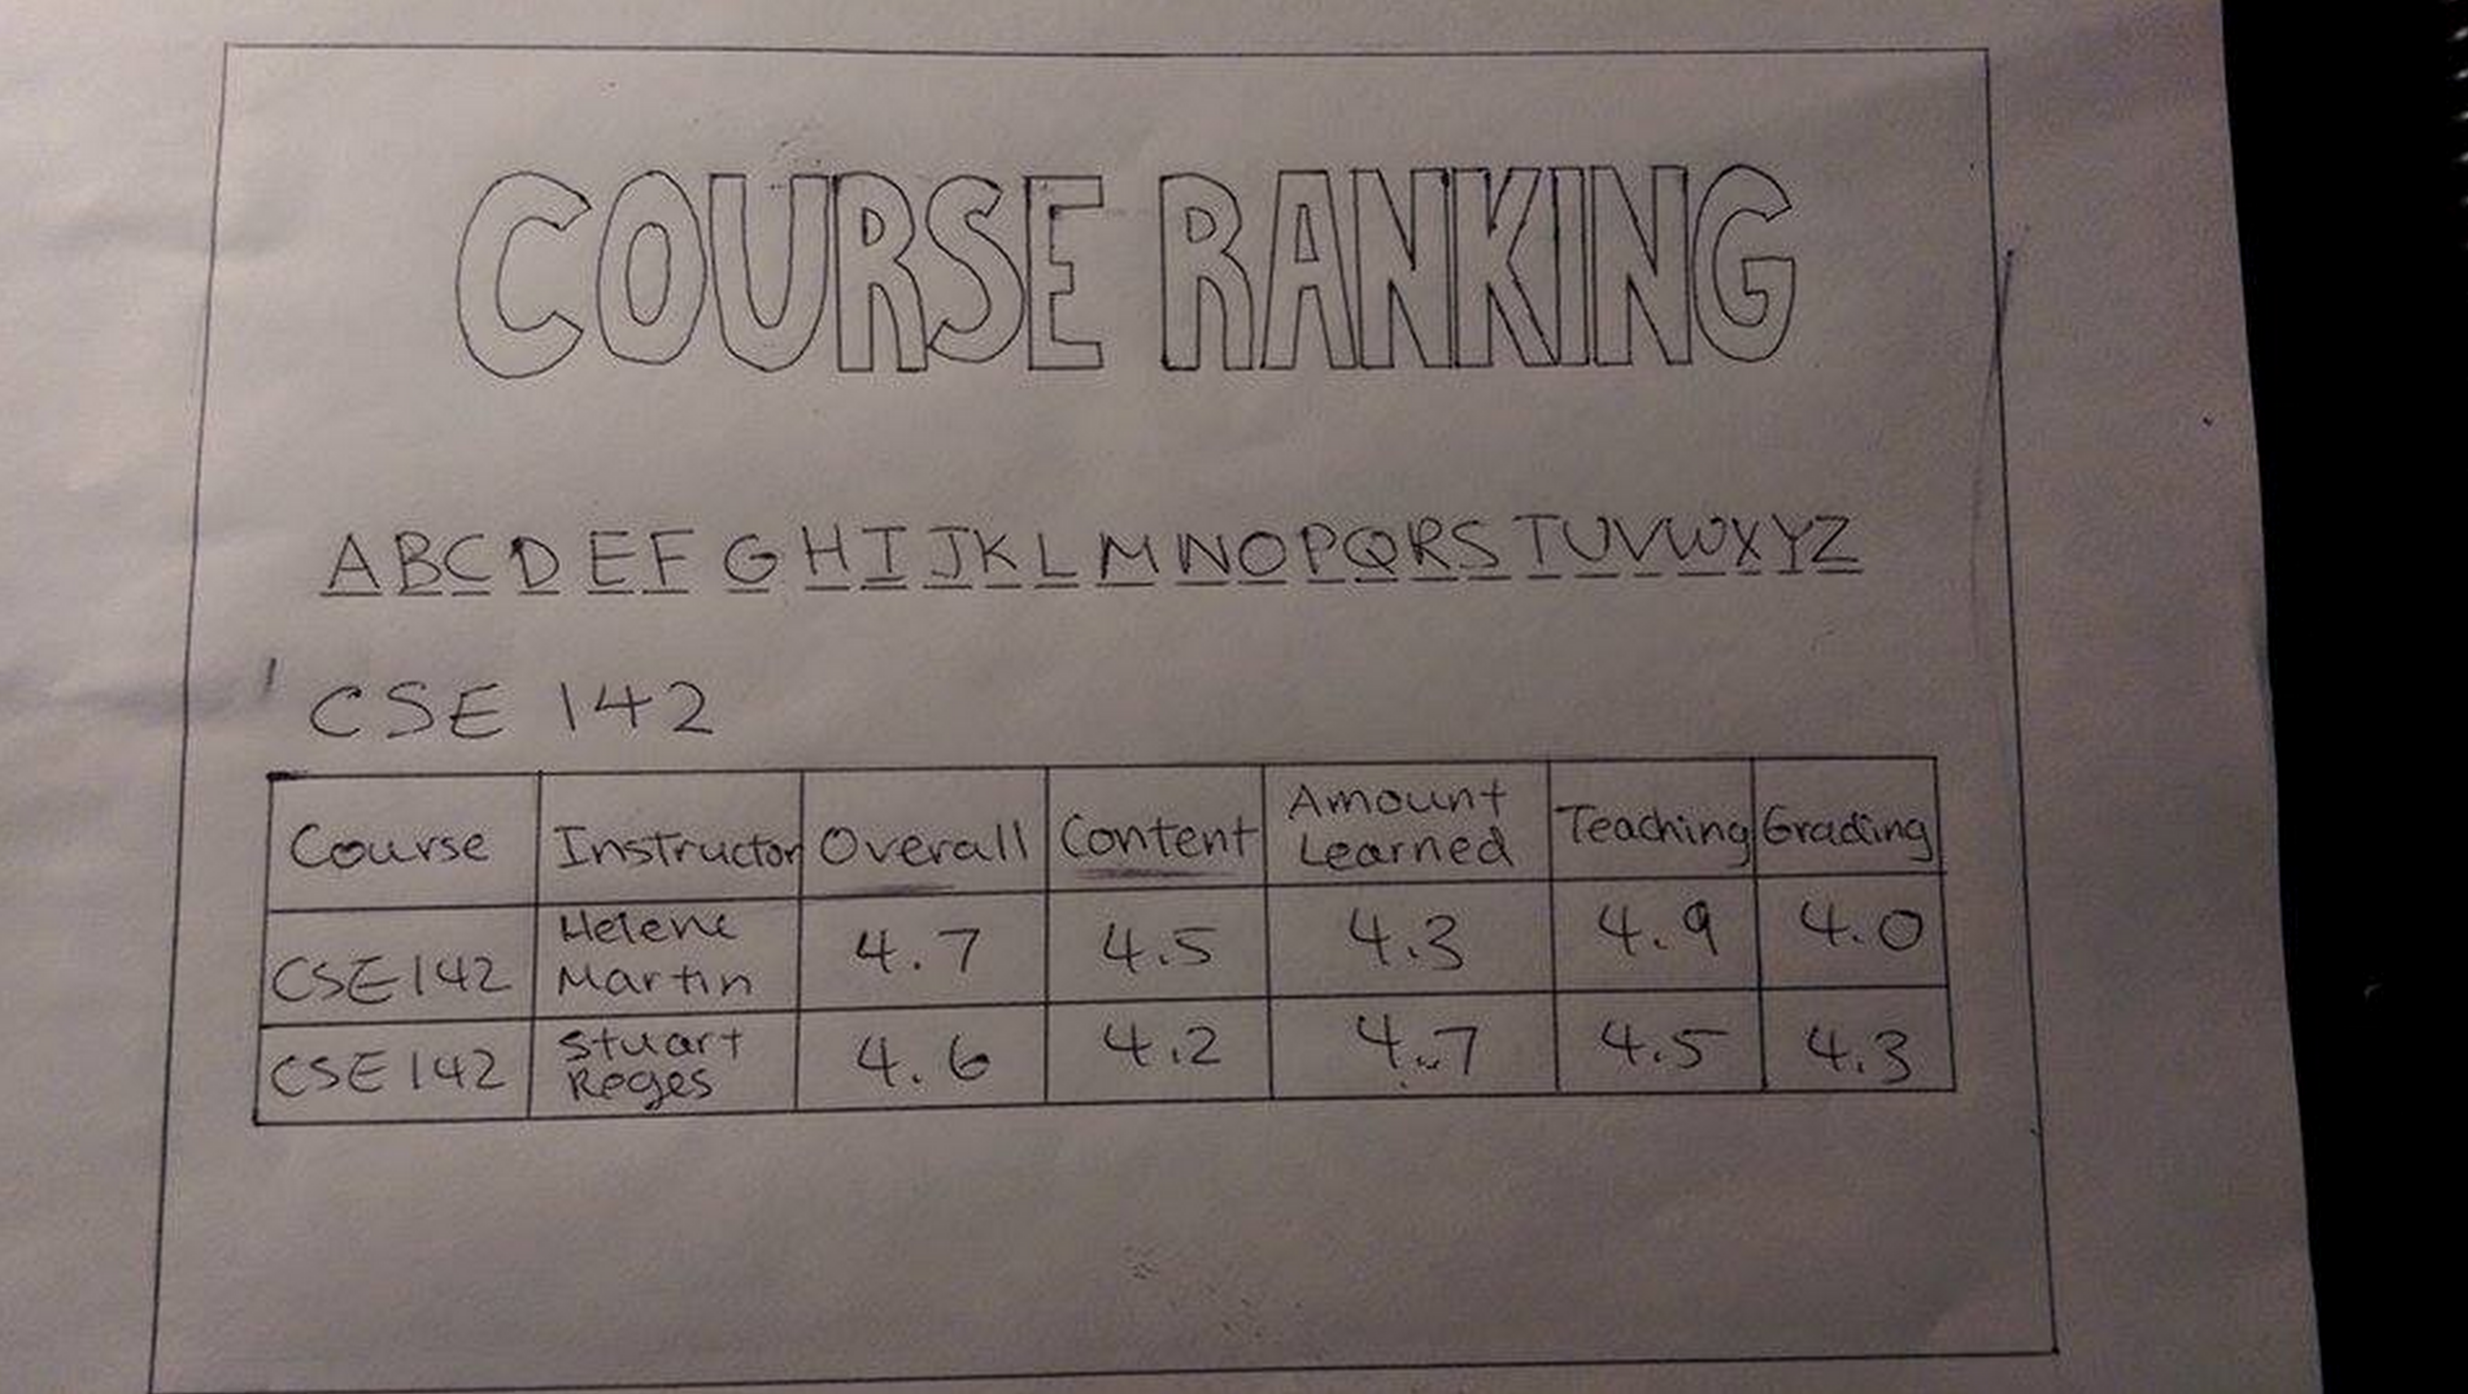
\includegraphics[width=\textwidth]{4.png}
\end{center}

We also realized that our visualization wouldn't be very helpful for a student who was searching for courses. For example, what if a student could take any computer science course, and was searching for the best one? Consequently, we decided allowing a users to sort the columns would be a good feature to have. This interaction technique is helpful because sorting is a common operation performed on datasets like ours where the goal is to compare multiple things. For example, if a student wanted to pick the best overall course, or the course with the best content, or so on, they would be able to do so.

\end{document}
